\documentclass[a4paper,10pt]{article}
\usepackage[utf8x]{inputenc}
\usepackage{graphicx}

%opening
\title{Exploring Your Favorite Corpus with The Topic Browser}


\begin{document}

\maketitle

\begin{abstract}
The Topic Browser is an open-source\footnote{Licensed under the terms of the
Affero General Public License, version 3.}  web application for interactive
exploration and visualization of topics and documents. Mallet LDA output is used
as input. We explain why such a tool is warranted, what it is capable of, and
how to use it to explore the corpus (or topic model) of your choice.
\end{abstract}

\section{Why?}
\subsection{Topic models are neat...}
Since their introduction in 2003, LDA-based topic models have been extended to
account for time, authors, citations, multiple languages, etc. [][][][][]
Baseline LDA generates a topic assignment per (non-stop) token -- a massive
output in the gigaword era. Humans are incapable of fully assimilating the
resulting models unaided, calling for more effective means of characterizing and
visualizing the output. 

Previous visualization attempts....

Why they fail





\subsection{...but their output is hard for humans to digest}
\subsection{Topics aren't isolated entities, but form a network in combination
with documents, words, authors, etc.}
\subsection{This network is implied by a topic model, but generally not made
explicit (?)}
\subsection{More informative}
Experience suggests that an explicit representation of the relationships between
all entities modeled and makes topic model output more informative and usable.
[We're in the process of formally validating this claim.]

\section{What?}
The Topic Browser is an open-source web application for interactive exploration
and visualization of document collections. 

\subsection{Entities}
\begin{figure}[ht]
 \centering
 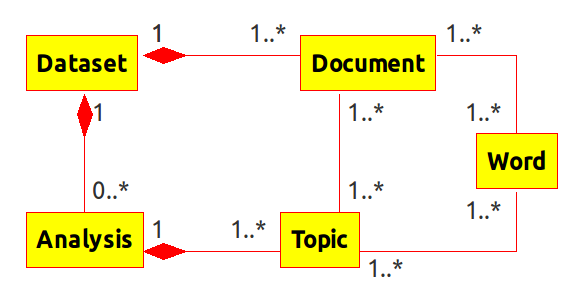
\includegraphics{topic_browser_object_model_transparent.png}
 % topic browser object model transparent.png: 582x293 pixel, 96dpi, 15.40x7.75
cm, bb=0 0 436 220
 \caption{The Topic Browser object model}
 \label{fig:object_model}
\end{figure}



All entities implied by topic model output are first-class citizens in the Topic
Browser. 
Dataset->Document
Analysis->Topic
Word

\subsection{Topics}

\subsection{Documents}

\subsection{Words}

\subsection{Metrics}
topic, topic-topic, document, document-document

\subsection{Charts}

\subsection{Topic ``Maps"}
With topic-to-topic relationships described by means of pairwise topic metrics,
graph-based visualization of the topic space becomes straightforward. In our
current implementation, we construct a topic graph G = (N, E) as follows:
\begin{itemize}
\item $N$ is a set of $|T|$ nodes such that $\forall_{t\in T} weight(N_{t}) =
\tau(t)$ where $\tau$ is a topic metric.
\item $E$ is a set of $|T|^2$ edges such that $\forall_{t\in T}\forall_{u\in T}
weight(E_{t,u}) = \mu(t,u)$ where $\mu$ is a pairwise topic metric.
\end{itemize}

We use the Gephi Toolkit\footnote{http://www.gephi.org} to generate such graphs
and render them as images.
\begin{figure}
\begin{center}
 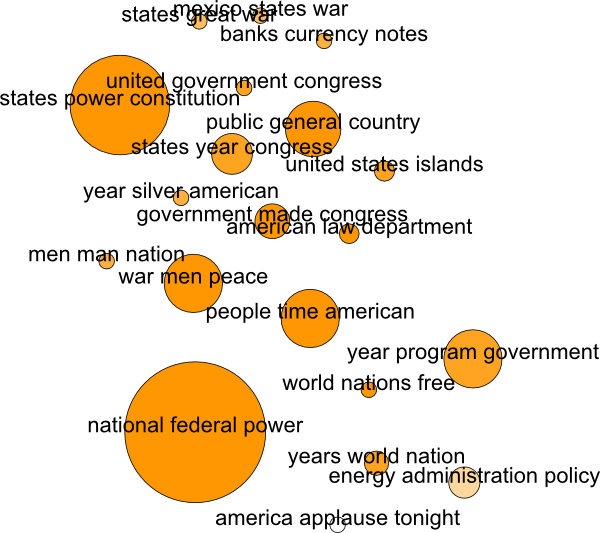
\includegraphics[width=200px,keepaspectratio=true]{./topic_map_example.png}
\caption{}
\end{center}
\end{figure} 
% \begin{center}
%  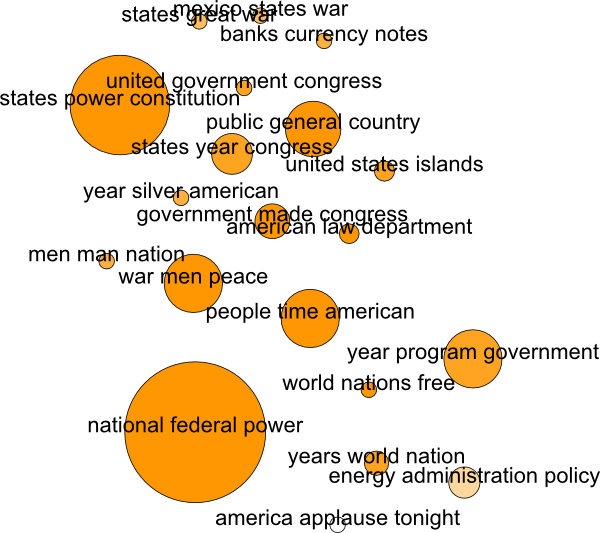
\includegraphics[width=200px,keepaspectratio=true]{./topic_map_example.png}
%  % topic_map_example.png: 600x533 pixel, 57dpi, 26.76x23.77 cm, bb=0 0 759 674
% \end{center}

\subsection{Topic Name Schemes}
As LDA does not assign names to the topics it generates, automatic generation of
topic names is of interest to researchers wishing to make topic models
human-usable. Research in this area is ongoing (CITATION???). In order to
facilitate investigations in this area, we equipped the Topic Browser with a
fully pluggable topic naming system. Any number of topic name schemes can be
used to produce names for all topics in an analysis. Within the user interface
users can select a name scheme, which is then reflected throughout the
interface. By default we use ''Top2`` (the name is a concatenation of the two
words with the highest $P(w|z)$ for a given topic $z$), but any number of
alternative schemes can be imagined and implemented. (MAYBE SHOW TF-ITF?)

\section{Backend Mechanics}
SHOW DEPENDENCY GRAPH?
Automatically turning a raw document collection into an interactive browsing
experience requires extensive preprocessing. Documents must be converted into a
representation accepted by the topic model learner. Topics must then be inferred
and model output indexed. Additionally, metrics must be computed, topic names
generated, and graphs rendered before they become accessible via the user
interface. Unsurprisingly, the dependencies in the import process form a DAG. To
improve the efficiency and usability of the data import pipeline we built a
command-line frontend based on the \verb/doit/ task automation tool, written in
Python.\footnote{http://doit.sourceforge.net/}

\subsection{Using The Build System}
The main \verb/doit/ build script is \verb/dodo.py/. Some example invocations:
\begin{itemize}
 \item \verb/dodo.py/: Builds all targets
 \item \verb/dodo.py list/: Lists the available top-level tasks (sub-tasks are not displayed)
 \item \verb/dodo.py clean -c mallet/: Cleans the Mallet files

\end{itemize}

% Useful commands:
%  dodo.py list #Lists the available top-level tasks (sub-tasks are not displayed)
%  dodo.py #Builds everything!
%  dodo.py clean -c mallet #Cleans the mallet files
%  dodo.py metrics #Computes all metrics
%  dodo.py topic_metrics #Computes just the topic metrics
%  dodo.py topic_metrics:document_entropy #Computes just the document entropy topic metric
%  dodo.py clean topic_metrics:document_entropy #Cleans just the document entropy topic metric
%
%NOTE: probably necessary to do 'dodo.py forget' when switching between datasets/analyses.

how to set different datasets

\subsection{Adding Support For Your Dataset}
The \verb/build/ Python module contains dataset-specific import scripts. Generally, a sub-module contains the scripts for a particular dataset. The scripts for the default State of the Union Addresses dataset, for example, reside in \verb/build.state_of_the_union/. The main build file for the dataset is \verb#build/state_of_the_union/state_of_the_union.py#. This file is referenced within the root \verb/dodo.py/ build script by setting the \verb/build/ variable:
\begin{verbatim}
 build = "state_of_the_union/state_of_the_union"
\end{verbatim}

At a minimum, the dataset-specific build file should contain the following:
\begin{itemize}
 \item Declaration of \verb/dataset_name/ variable.
   \newline Example: \verb/dataset_name = "state_of_the_union"/.
 \item Declaration of \verb/dataset_description/ variable.
   \newline Example: \verb/dataset_description = "State of the Union Addresses 1790-2010"/.
 \item Definition of \verb/copy_and_transform_dataset/ \verb/doit/ task. Example:
\begin{verbatim}
def task_copy_and_transform_dataset():
  task = dict()
  task['actions'] = [
    (extract_state_of_the_union,
    [dataset_dir+'/'+chron_list_filename,
     dataset_dir+'/'+addresses_filename,
     files_dir]
    )
  ]
  task['clean'] = [
    'rm -rf '+files_dir
  ]
  task['uptodate'] = [os.path.exists(files_dir)]
  return task
\end{verbatim}

\end{itemize}





\end{document}
